\clearpage
\section{Control of \zInv\ background \label{app:zInvBgControl}}


An accurate prediction of the \zInv\ background is a crucial part 
of the analysis. Up to five control samples may be used 
to predict the \zInv\ background: \mj, \mmj, \ej, \eej and \gj. 
In previous versions of this analysis only the \zmmj and 
\gj to predict the \zInv\ background. The single
lepton control samples also provide \wj enriched samples to predict
\zInv\ with significantly higher statistical power. 
Several closure tests are used to probe the 
systematcs related to the predictions of the \zInv\ background
and are described below.

The data-driven tests are described in full in Sec.~\ref{sec:closure-tests},
Those relevant for the \zInv\ prediction are the \mmj to \gj
which probes the photon prediction, the \mj to \mmj which probes the
prediction from W and the \mj to \gj which probes vector boson prediction 
using the photon sample. In addition to these, a test to probe the effect
of W polarisation on experimental acceptance, $\mu^+$ + jets to $\mu^-$ + jets,
is described below. Using data from $8\TeV$, 
these closure tests are shown in Fig.~\ref{fig:wpolCT}.
This shows that the predictions of \zInv\ from
all control samples are consistent within statistical 
uncertainty with no bias or trend. 


The production mechanism of W from pp collisions means
high $p_T$ W bosons are predominantly left handed \cite{WPol}.  
For high $p_T$ bosons, this implies that $W^+$ will decay 
to the left handed neutrino along its direction of motion while 
the lepton will be backward. The opposite behaviour is
expected for the $W^-$. The lepton will therefore be more boosted (and
the neutrino less boosted) in $W^+$ decays than $W^-$ decays.  This
leads to a larger number of $W^+$ decays in the single lepton control
regions (which relies on the lepton $p_T$ for acceptance) than in the
signal region (which relies on the neutrino $p_T$ for acceptance). In
order to understand if this leads to a bias in the prediction of the
$W$ and unpolarised \zInv\ background in the signal region when using
a single lepton control region a closure test from $\mu^+$ + jets to
$\mu^-$ + jets will be added (shown in Fig.~\ref{fig:wpolCT}. 

\begin{figure}[h!]
 \begin{center}  
  \subfigure[Closure tests for $\le3$ jets]{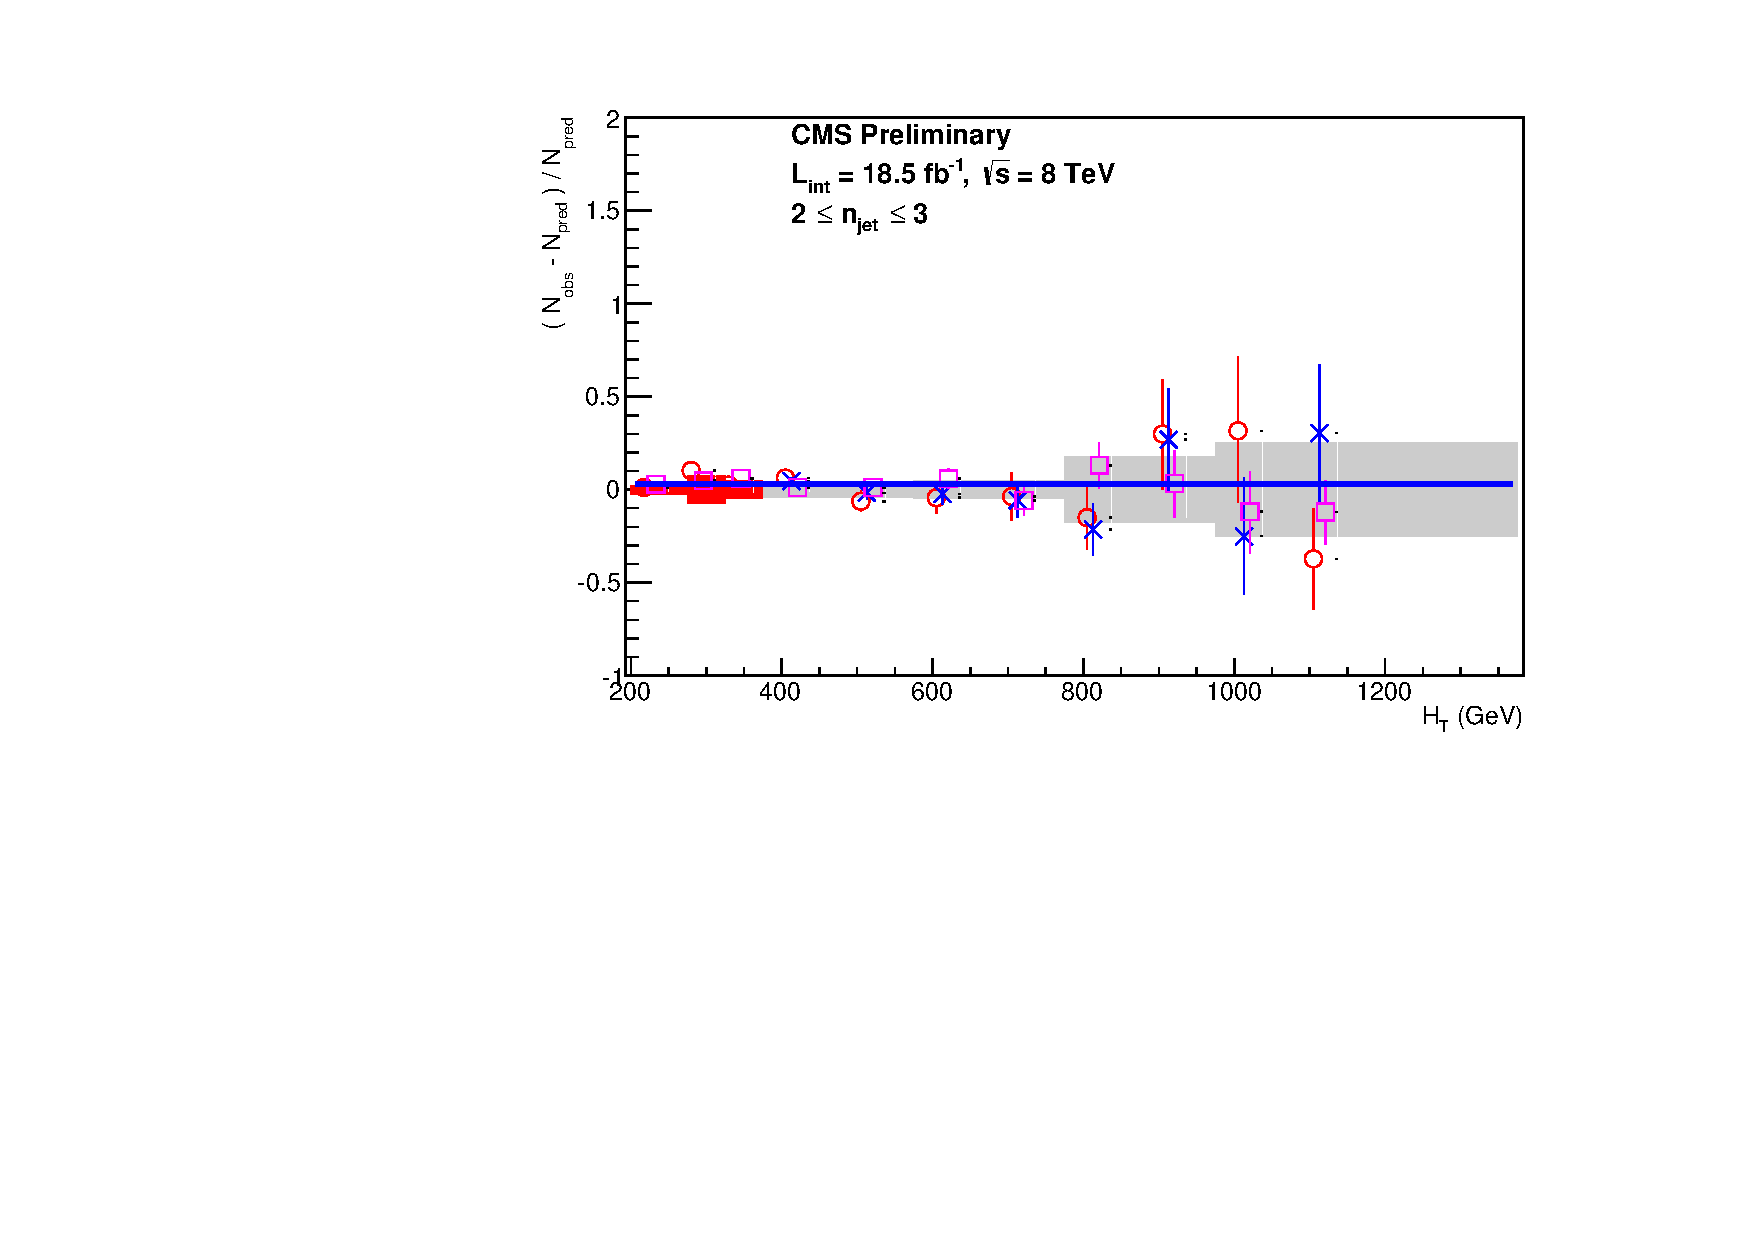
\includegraphics[width=0.5\textwidth]{figures/wPol/summaryLe3J.pdf}} ~~
  \subfigure[Closure tests for $\ge4$ jets]{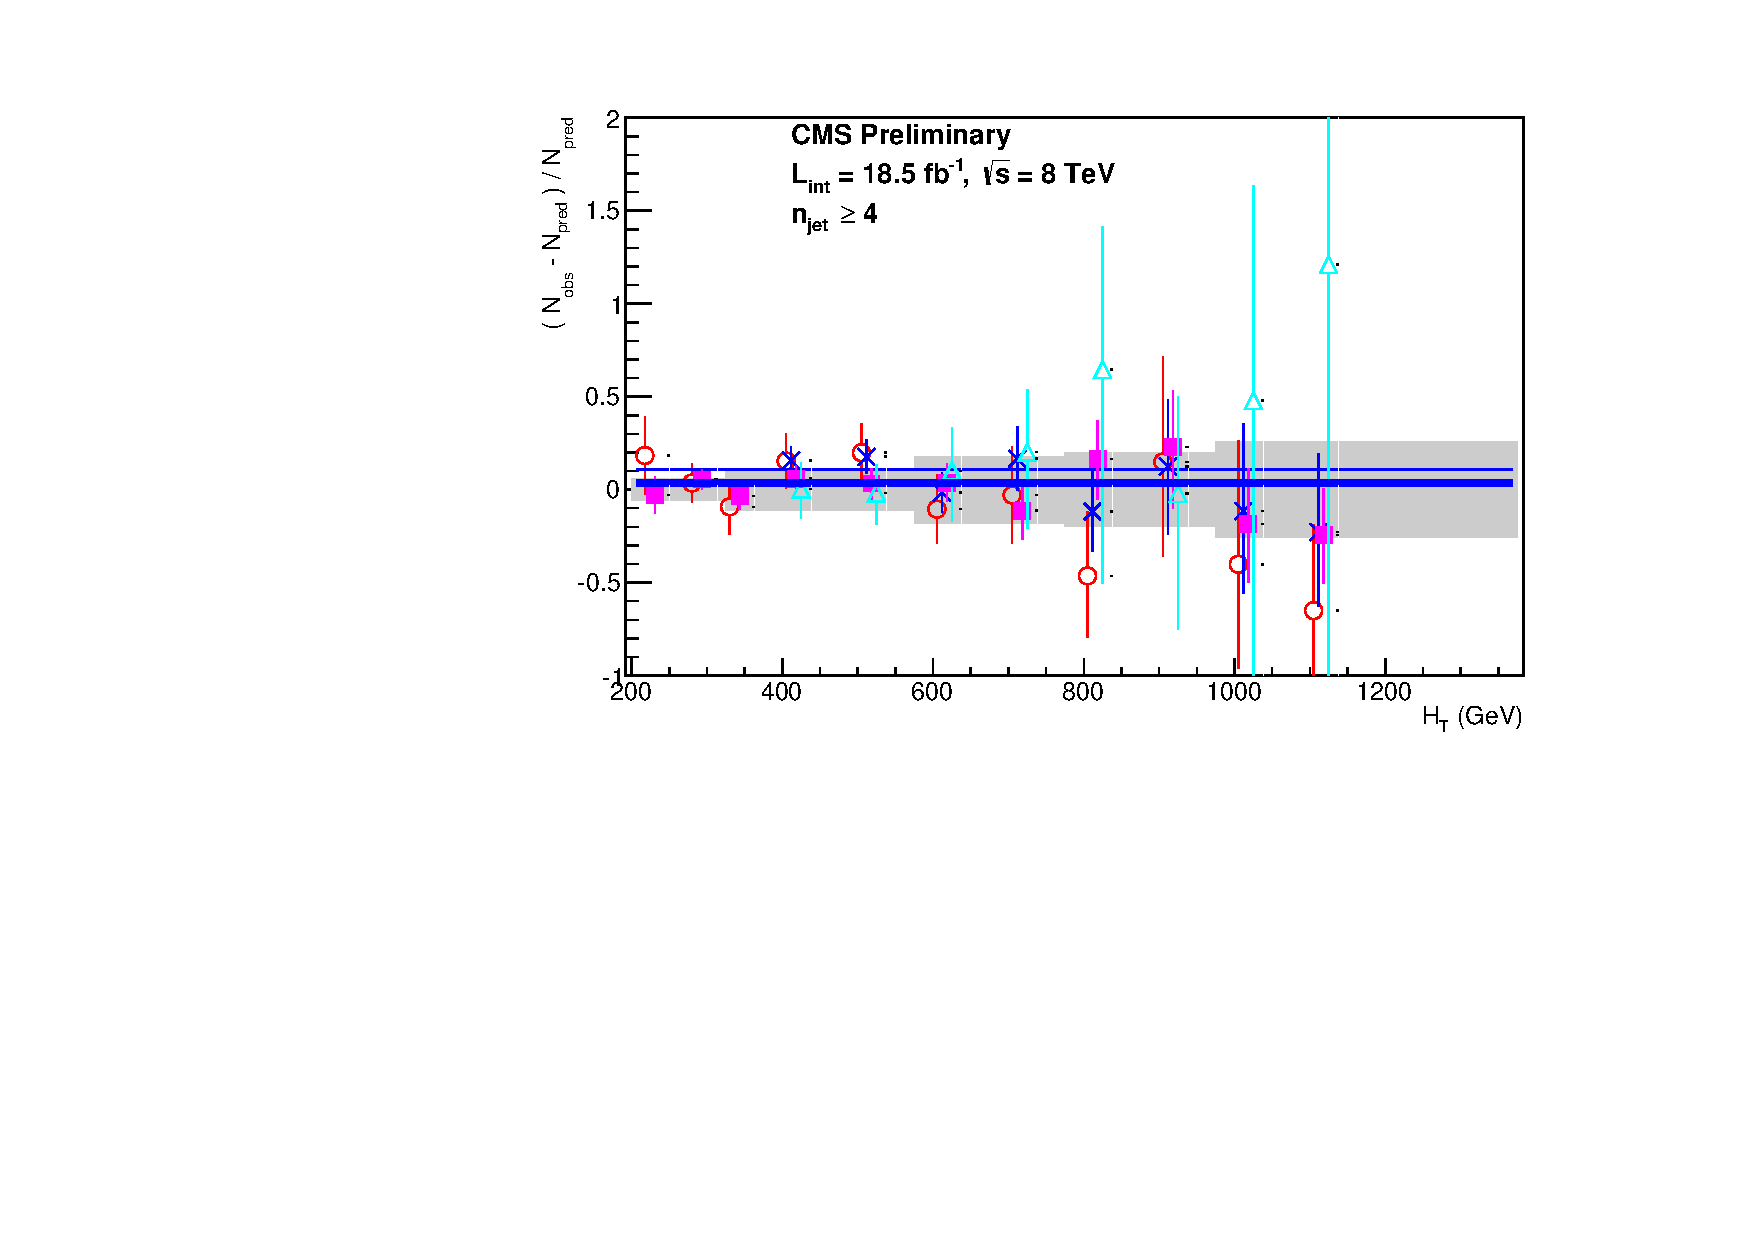
\includegraphics[width=0.5\textwidth]{figures/wPol/summaryGe4J.pdf}}
  \caption{Closure tests that probe the effects of W polarisation on
    experimental acceptance. The red circles correspond to the \mj to
    \mmj closure test, the blue crosses correspond to the \mj to \gj closure test,
    the pink squares correspond to the $\mu^+$ + jets to $\mu^-$ + jets 
    closure test and the turquoise triangles correspond 
  to the \mmj to \gj closure test.}
  \label{fig:wpolCT}
 \end{center}
\end{figure}          
